\documentclass[a4paper,11pt]{book} 

\usepackage[T1]{fontenc}
\usepackage[utf8]{inputenc}
\usepackage[spanish]{babel}

\usepackage{graphicx}

\usepackage{colortbl}
\usepackage{color}

\usepackage{hyperref}

\usepackage[margin=1in]{geometry}
\pagestyle{plain}

%\usepackage{fancyhdr} 
%\usepackage{lastpage}
%\usepackage{float} 
%\floatstyle{boxed} 
%\restylefloat{figure} 
%\pagestyle{fancy}

\definecolor{orange}{RGB}{255,127,0}
\setcounter{secnumdepth}{4}
\setcounter{tocdepth}{3}
\title{\textcolor{orange}{Informe Trabajo Final}}
\author{Grupo Lovaisa-Gomez \\ Facultad de Ciencias Físicas , Exactas y
Naturales\\ Sistemas de Computación}

\begin{document}

%\lhead{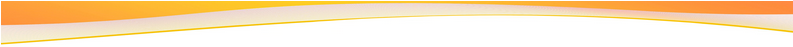
\includegraphics[width=1\textwidth]{../img/encab.png}}
%\lfoot{{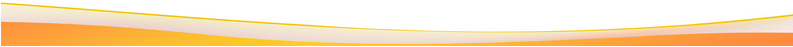
\includegraphics[width=1\textwidth]{../img/pie.png}}}
%\rfoot{\thepage}

\maketitle
\tableofcontents


\chapter{\textcolor{orange}{INTRODUCCION}}

\newpage
\section{\textcolor{orange}{Introducción}}
El siguiente informe refleja el trabajo realizado para el desarrollo de un
sistema de monitoreo y registro de datos multiplataforma correspondiente a la
materia Sistemas de Computación. El objetivo principal de este trabajo es
realizar un sistema formado por tres subsistemas que interactuan por
conexiones Serial y Ethernet. El primer subsistema consiste en una plataforma
basada en un microcontrolador Atmel - Arduino(R) Mega 2560 - para la
adquisición de datos en Tiempo Real. Este consta de un sensor de temperatura
conectado a un puerto del ADC de la placa el cual envía los valores medidos de
temperatura al servidor por medio de una conexión Serial sin ningun tipo de
procesamiento o ajuste de señal para evitar cualquier demora en la recepción de
los datos. 
En la etapa intermedia los datos recibidos por el servidor, que
corre sobre una arquitectura x86, son procesados para obtener un formato y
escala legible por humanos (Grados Celsius), para luego ser almacenados en una
base de datos mysql. La recepción de datos se realiza en un proceso
independiente que a medida que los datos van arrivando los almacena en un buffer
circular en memoria compartida. Luego, otro proceso va recolectando los datos
almacenados en el buffer los escala y almacena en la base de datos.
En la etapa final se cuenta con una placa iMX53 con un SO Linux embebido que da
soporte a una aplicación con interfaz gráfica desarrollada en Qt utilizada para
acceder y presentar los datos almacenados en la base de datos del servidor. La
conexión de la iMX53 y el servidor x86 se realiza mediante Ethernet. Desde la
aplicación gráfica puden establecerse niveles de temperatura Max y Min que
activarán indicaciones visuales en cada caso.   
% === Figura ====
\begin{figure}[h!]
 \begin{center}
  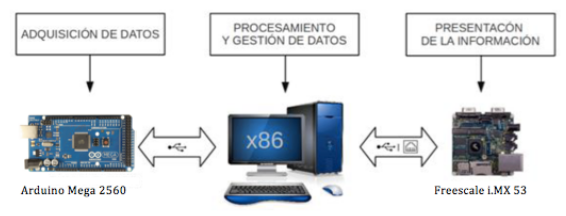
\includegraphics[width=0.5\textwidth,keepaspectratio=true]{../img/fig1.png}
  \caption{Esquema general del sistema}
  \label{fig:esquema}
 \end{center}
\end{figure}
% ===============
Se implementaron métodos de toma de requerimientos , estimaciones ,
diseño de arquitectura, implementación, testing, procedimientos y técnicas
de Ing del Software.

\section{\textcolor{orange}{Desarrollo}}
Durante el desarrollo del trabajo se relizaron los siguientes documentos de
diseño

\vspace{1cm}

\begin{table}[!h]
\begin{center}
\begin{tabular}{|c|c|c|}
\hline
\rowcolor[RGB]{255,127,0} Acrónimo & Documento \\
%\hline
%SCMP & Software Configuration Managment Plan & yyy\\
\hline
SRS & Software Requerimients Specification \\
\hline
ADD & Arquitecture Design Documentation \\
\hline
SSD & Software Design Description \\
\hline
STD & Software Test Documentation \\
\hline
%SRN & Software Release Note & yyy\\
%\hline
%SPMP & Software Project Management Plan & yyy\\
%\hline
\end{tabular}
\end{center}
\end{table}

\chapter{\textcolor[gray]{.2}{SRS - SOFTWARE REQUERIMENTS SPECIFICATION}}

%\newpage
%\section{\textcolor{orange}{Historial de Versiones}}
%\begin{table}[H]
%\begin{center}
%\begin{tabular}{|c|c|c|c|}
%\hline
%\rowcolor[RGB]{255,127,0} Vesión & Fecha & Descripción de Cambios & Autor\\
%\hline
%1.0 & 09/07/2013 & Primera Versión & Gomez P.\\
%\hline
%1.1 & 01/12/2013 & LEL, Escenarios y Tarjetas CRC & Lovaisa V.\\
%\hline

%\end{tabular}
%\end{center}
%\end{table}
%\newpage

\newpage
\section{\textcolor[gray]{.2}{Historial de Versiones}}
\begin{table}[h!]
\begin{center}
\begin{tabular}{|c|c|c|c|}
\hline
\rowcolor[gray]{.8} Vesión & Fecha & Descripción de Cambios & Autor\\
\hline
1.0 & 09/07/2013 & Primera Versión & Gomez P.\\
\hline
1.1 & 01/12/2013 & LEL, Escenarios y Tarjetas CRC & Lovaisa V.\\
\hline
\end{tabular}
\end{center}
\end{table}

%\section{\textcolor{orange}{Página de Aprobaciones}}
%A continuación se listan las personas de las cuales se requiere la aceptación de cualquier cambio mayor de este documento.
%\begin{enumerate}
 % \item Estas aprobaciones no son necesarias si el cambio es menor.
 % \item Estas aprobaciones son necesarias si el cambio es realizado por alguna persona distinta de ellas.
%\end{enumerate}
%\begin{table}[h!]
%\begin{center}
%\begin{tabular}{|c|c|c|c|}
%\hline
%\rowcolor[RGB]{255,127,0} Nombre & Cargo & Fecha & Firma\\
%\hline
%Lovaisa Valeria & Resp. Ingeniería de Requerimientos & 09/07/2013 & \\
%\hline
%Gomez Pablo & Resp. Suplente & 09/07/2013 & \\
%\hline
%\end{tabular}
%\end{center}
%\end{table}

\section{\textcolor[gray]{.2}{Página de Aprobaciones}}
A continuación se listan las personas de las cuales se requiere la aceptación de cualquier cambio mayor de este documento.
\begin{enumerate}
  \item Estas aprobaciones no son necesarias si el cambio es menor.
  \item Estas aprobaciones son necesarias si el cambio es realizado por alguna
  persona distinta de ellas.
\end{enumerate}
\begin{table}[h!]
\begin{center}
\begin{tabular}{|c|c|c|c|}
\hline
\rowcolor[gray]{.8} Nombre & Cargo & Fecha & Firma\\
\hline
Lovaisa Valeria & Resp. Ingeniería de Requerimientos & 09/07/2013 & \\
\hline
Gomez Pablo & Resp. Suplente & 09/07/2013 & \\
\hline
\end{tabular}
\end{center}
\end{table}


\newpage
\section{\textcolor[gray]{.2}{Introducción}}
\subsection{\textcolor[gray]{.2}{Propósito y Alcance}}

Este documento cubre el proceso de elicitación de requerimientos del sistema
de monitoreo y registro de datos multipropósito. Este SRS tiene como objetivo
establecer cuales son los requerimientos del sistema a nivel de usuario, como
así también a nivel de sistema (requerimientos detallados). 

\subsection{\textcolor[gray]{.2}{Acrónimos y Glosario}}
\begin{table}[h!]
\begin{center}
\begin{tabular}{|c|c|}
\hline
\rowcolor[gray]{.8} Acrónimo & Descripción \\
\hline
SRS & Software Requirements Specification - Especificación de Req. de Software \\
\hline
SRM & Software Requirements  Manager – Responsable de requerimientos del sistema\\
\hline
\end{tabular}
\end{center}
\end{table}

\subsection{\textcolor[gray]{.2}{Herramientas Necesarios}}
\begin{table}[h!]
\begin{center}
\begin{tabular}{|c|p{100mm}|}
\hline
\rowcolor[gray]{.8} Programa & Propósito \\
\hline
Planilla de Cálculos Generica & Para llevar en control de la trazabilidad
de requermientos usr. vs req. de sistema y de req. vs casos de uso.\\
\hline
Dia & Software para la creación de diagramas UML\\
\hline
Google-Drive & Software necesario para llevar el control de los requerimientos.\\
\hline
\end{tabular}
\end{center}
\end{table}

%\newpage
%\\section{\\textcolor[gray]{.2}{Roles}}
%\subsection{\textcolor[gray]{.2}{Responsables}}
%Las actividades de ingeniería de requerimientos del Sistema serán coordinadas en este proyecto por el Responsable de Requerimientos del sistema. (SRM). Este Rol debe ser asignado a alguno de los miembros del proyecto.
%El SRM será el responsable directo de las actividades de requerimientos del
%sistema, responder ante modificaciones en los mismos  y de mantener la documentación relacionada actualizada (Modificación de requerimientos , Modificación del sistema de trackeo).

%\subsection{\textcolor[gray]{.2}{Roles}}
%\begin{table}[!h]
%\begin{center}
%\begin{tabular}{|c|c|c|}
%\hline
%\rowcolor[gray]{.8} Rol & Nombre & Suplente\\
%\hline
%SRM & Lovaisa Valeria & Gomez Pablo\\
%\hline
%\end{tabular}
%\end{center}
%\end{table}

\newpage
\section{\textcolor[gray]{.2}{Requerimientos}}
\subsection{\textcolor[gray]{.2}{Listado de Requerimientos No Funcionales}}
\subsubsection{\textcolor[gray]{.2}{Requerimientos de apariencia
(Requerimientos de percepción)}}
\begin{enumerate}
\item Las interfaces gráficas deben estar elaboradas bajo el Framework Qt
\item El sistema debe brindar una interfaz gráfica basada en ventanas ,
formularios y menues.
\item El sistema debe visualizarse en Español (Latinoamérica – Argentina).
\end{enumerate}


\subsubsection{\textcolor[gray]{.2}{Requerimientos de facilidad de utilización
(Requerimientos de usabilidad)}}
\begin{enumerate}
\item El sistema debe permitir el teclado como dispositivo de entrada.
\item El sistema debe permitir el mouse como dispositivo de entrada.
\end{enumerate}

\subsubsection{\textcolor[gray]{.2}{Requerimientos de velocidad y latencia
(Requerimientos de desempeño)}}
\begin{enumerate}
\item El sistema debe tener un tiempo de respuesta menor o igual a un (1)
segundo.
\item El sistema debe tener acceso a una red LAN Ethernet de velocidad 100 Mbps.
\end{enumerate}

\subsubsection{\textcolor[gray]{.2}{Requerimientos de confiabilidad y
disponibilidad (Requerimientos de desempeño)}}
\begin{enumerate}
\item El sistema debe estar disponible mínimo un 99\% del tiempo en el que este
se encuentre en ejecución.
\end{enumerate}

\subsubsection{\textcolor[gray]{.2}{Requerimientos de capacidad (Requerimientos de
desempeño)}}
\begin{enumerate}
\item El sistema debe tener acceso a mínimo 512 KB de memoria RAM disponibles
para la ejecución de su módulo de presentación gráfica.
\item El sistema debe tener acceso a mínimo 512 KB de memoria RAM disponibles
para la ejecución de su módulo de manejo y registro de datos.
\item El sistema debe tener acceso a mínimo un procesador de 1 GHz para la
ejecución de su módulo de presentación gráfica.
\item El sistema debe tener acceso a mínimo un procesador de 1.2 GHz para la
ejecución de su módulo de manejo y registro de datos.
\end{enumerate}
 
\subsubsection{\textcolor[gray]{.2}{Requerimientos de ambiente físico esperado
(Requerimientos operacionales y ambientales)}}
\begin{enumerate}
\item El módulo de adquisición de datos debe poder ejecutarse un
microcontrolador arduino MEGA2560 situado fisicamente en sala de ambiente
controlado (Valores sensados : Humedad y Temperatura).
\item El módulo de manejo y registro de datos debe poder ejecutarse en un
servidor de arquitectura x86.
\item El módulo de presentación de datos debe poder ejecutarse en una placa de
desarrollo iMx53 situada fisicamente en un lugar de facil acceso en sala de
ambiente controlado.
\end{enumerate}

\subsubsection{\textcolor[gray]{.2}{Requerimientos de acceso (Requerimientos de
seguridad)}}
\begin{enumerate}
\item El sistema debe registringir el acceso al módulo de manejo y registro de
datos en el servidor mediante usuario y contraseña. 
\item El sistema debe contar con diferentes niveles de privilegios en el acceso
a los módulos de presentación de datos y manejo/registro de datos.
\end{enumerate}

\subsubsection{\textcolor[gray]{.2}{Requerimientos de integridad (Requerimientos
de seguridad)}}
\begin{enumerate}
\item El sistema no debería permitir la modificiación de variables de
configuración durante la adquisición de datos.
\end{enumerate}

\subsubsection{\textcolor[gray]{.2}{Requerimientos de privacidad (Requerimientos
de seguridad)}}
\begin{enumerate}
\item El sistema debería guardar los datos de acceso (usuario y contraseña) en
el equipo en que se esta ejecutando. 
\end{enumerate}

\subsubsection{\textcolor[gray]{.2}{Requerimientos de inmunidad
(Requerimientos de seguridad)}}
\begin{enumerate}
\item El sistema deberá verificar que todos los datos que el usuario ingrese
sean correctos.
\item El sistema deberá verificar que todos los datos que el administrador
ingrese sean correctos.
\end{enumerate}

\subsubsection{\textcolor[gray]{.2}{Requerimientos de cumplimiento
(Requerimientos legales)}}
\begin{enumerate}
\item El sistema debe ser entregado en la semana del 22 al 26 de Julio.
\end{enumerate}


\subsubsection{\textcolor[gray]{.2}{Requerimientos de legalidad (Requerimientos
legales)}}
\begin{enumerate}
\item El sistema no puede desarrollarse bajo herramientas obtenidas de forma
ilegal (Uso de seriales copiados, cracks, keygens, entre otros)
\end{enumerate}

\subsubsection{\textcolor[gray]{.2}{Requerimientos de estándares (Requerimientos
legales)}}
\begin{enumerate}
\item El código fuente del sistema debe estar debidamente documentado en
Español (Latinoamérica – Argentina)
\item El código debe ser desarrollado en C , C++ , Qt, mysql y debe seguir los
estándares involucrados en dicha tarea.
\end{enumerate}


\newpage
\section{\textcolor[gray]{.2}{Listado de Requerimientos Funcionales}}
El listado completo de requerimientos se encuentra gestionado en una planilla de
cálculo opensource en Google Drive.


\begin{table}[h!]
\begin{center}
\begin{tabular}{|c|p{100mm}|}
\hline
\rowcolor[gray]{.8} Descripción & Link \\
\hline
Listado Maestro de Requerimientos &
\url{https://docs.google.com/spreadsheet/ccc?key=0AuDVazeuJzKkdGN2bUZoVmRlM3EybHUwVS1zWXNWTlE#gid=0}\\
\hline
\end{tabular}
\end{center}
\end{table}

Con esta herramienta se realiza la documentación de todos los requerimientos
del sistema y la gestión de modificaciones en los mismos. Así también se logra
distribuir la planificación de trabajo logrando saber quien esta desarrollando
la implementación de cada uno de estos requerimientos en ese momento.
Los requerimientos de funcionales de usuario de dividen en grupos , como
muestra la siguiente tabla.

\begin{table}[h!]
\begin{center}
\begin{tabular}{|c|c|}
\hline
\rowcolor[gray]{.8} Tipo & Descripción \\
\hline
Adquisición & Req. relacionados a la forma de obtención de los
datos.\\
\hline
Manejo y Registro & Req. relacionados a la forma en que el servidor administra
los datos\\
\hline
Presentación & Req. relacionados a la forma en que se muestran los datos al
usuario.\\
\hline
\end{tabular}
\end{center}
\end{table}

En la herramienta de gestión de requerimientos se colocarán los tags
correspondientes para cada tipo de requerimientos.
%Las asociaciones entre requerimientos y requerimientos se encuentran
%documentados en la matriz de trazabilidad.

%\begin{table}[!h]
%\begin{center}
%\begin{tabular}{|c|p{100mm}|}
%\hline
%\rowcolor[gray]{.8} Descripción & Link \\
%\hline
%Matriz de Req vs Req &
%\url{https://docs.google.com/spreadsheet/ccc?key=0AuDVazeuJzKkdFJEbkpaVV91el9EM0NSMVFYendXdWc#gid=0}\\
%\hline
%\end{tabular}
%\end{center}
%\end{table}

Las asociaciones entre diagramas de casos de uso y requerimientos se encuentran
documentados en la herramienta de gestión de requerimientos. 

%\begin{table}[!h]
%\begin{center}
%\begin{tabular}{|c|p{100mm}|}
%\hline
%\rowcolor[gray]{.8} Descripción & Link \\
%\hline
%Matriz de Req vs UCs &
%\url{https://docs.google.com/spreadsheet/ccc?key=0AuDVazeuJzKkdHR3Mm5sQUpXYldUOTlHT0JIX1l6bWc#gid=0}\\
%\hline
%\end{tabular}
%\end{center}
%\end{table}

\newpage
\subsection{\textcolor[gray]{.2}{Tabla de requerimientos - Lista maestra de
requerimientos}} 
\begin{table}[h!]
\begin{center}
\begin{tabular}{|p{30mm}|p{70mm}|p{30mm}|}
\hline
\rowcolor[gray]{.8} Requerimiento N & Descripción & Tipo \\
\hline
RQX001 & El arduino mega 2560 debe poder enviar datos tomados desde el sensor
de temperatura y humedad al servidor por medio de una conexión serial  u
Ethernet & Adquisición\\
\hline
RQX002 & El sistema de adquisición y registro de datos de temperatura debe poder
capturar datos con un intervalo máximo de 1 segundo & Adquisición \\
\hline
RQX003 & Los parámetros de configuración del modulo de Adquisición deben poder
configurarse desde el servidor de manejo y registro de datos & Adquisición \\
\hline
RQX004 & El modulo de adquisición debe poder identificarse con el servidor para
iniciar el envió de datos & Adquisición \\
\hline
RQX005 & El sistema de manejo y registro de datos debe poder conectarse con uno
o varios modulos de adquisicion de datos por medio de una conexión serial u
Ethernet & Manejo y Registro \\
\hline
RQX006 & El sistema de registro y manejo de datos de temperatura debe poder
manupular los  datos convirtiendolos a un formato legible para seres humanos &
Manejo y Registro\\
\hline
RQX007 & El sistema de registro y manejo de datos de temperatura debe poder
registrar y administrar todos los dispocitivos de adquisicion que se identifican
& Manejo y Registro\\
\hline
RQX008 & El sistema de registro y manejo de datos de temperatura debe poder
almacenar los datos recibidos y convertidos en una base de datos My SQL & Manejo
y Registro\\
\hline
RQX009 & El sistema de registro y manejo de datos de temperatura debe poder
registrar en una base de datos todos los dispocitivos de adquision que se
conecten al servidor & Manejo y Registro \\
\hline
RQX010 & El sistema de registro y manejo de datos de temperatura debe poder 
enviar via conexión Ethernet cada 1 segundo los datos al modulo de presentacion
& Manejo y Registro\\
\hline
\end{tabular}
\end{center}
\end{table}

\newpage

\begin{table}[h!]
\begin{center}
\begin{tabular}{|p{30mm}|p{70mm}|p{30mm}|}
\hline
\rowcolor[gray]{.8} Requerimiento N & Descripción & Tipo \\
\hline
RQX011 & El sistema de registro y manejo de datos de temperatura debe poder
enviar el promedió para diferentes intervalos de tiempo últimos 5, 15 y 60
minutos al modulo de presentación & Manejo y Registro\\
\hline
RQX012 & El sistema de registro y manejo de datos de temperatura debe poder
verificar los valores medidos se encuentren dentro de el rango establecido &
Manejo y Registro\\
\hline
RQX013 & El sistema de registro y manejo de datos de temperatura debe permitir
configuar los valores maximos y minimos & Manejo y Registro\\
\hline
RQX020 & El modulo de registro y manejo de datos de temperatura debe permitir a
un usuario adquierir privilegios de administrador mediante un password & Manejo
y Registro\\
\hline
RQX014 & El modulo de presentacion de datos debe poder conectarse con un
servidor via conecxion Ethernet & Presentación\\
\hline
RQX015 &  El modulo de presentacion de datos debe poder mostrar los datos de
temperatura enviados desde el servidor en al menos dos escalas distintas celsius
y farenheit & Presentación\\
\hline
RQX016 & El modulo de presentacion de datos debe poder indicar graficamente si
los valores de temperatura se encuentran fuera del rango permitido &
Presentación\\
\hline
RQX017 & El modulo de presentacion de datos debe permitir cambiar la direccion
ip del servidor & Presentación\\
\hline
RQX018 & El modulo de presentación de datos debe permitir a un administrador
seleccionar algún dispositivo de adquisición de datos conectado al servidor &
Presentación\\
\hline
RQX019 & El modulo de presentación de datos debe permitir a un administrador
acceder a las configuraciones por medio de usuario y contraseña & Presentación\\
\hline
\end{tabular}
\end{center}
\end{table}

\newpage
\subsection{\textcolor[gray]{.2}{Diagramas de Secuencia}}
\subsubsection{\textcolor[gray]{.2}{Adquisición, registro de datos y presentación de datos}}
% === Figura ====
\begin{figure}[h!]
 \begin{center}
  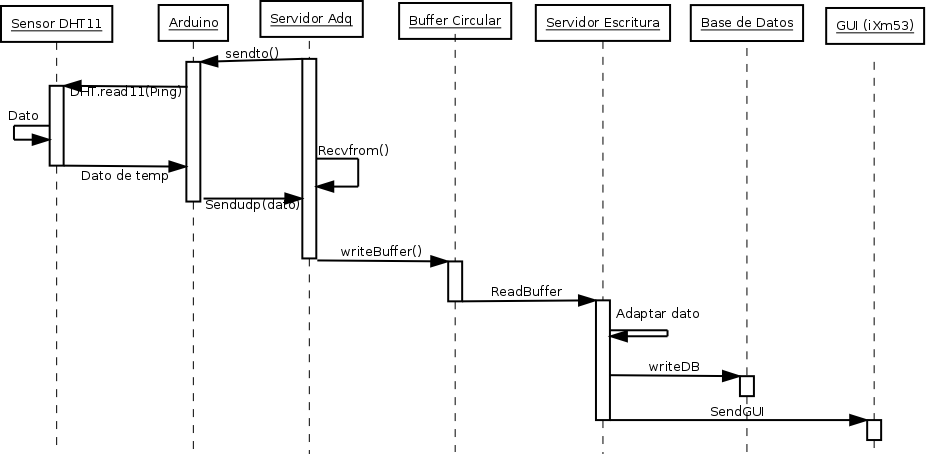
\includegraphics[width=1\textwidth,keepaspectratio=true]{img/Diagrama_secuencia.png}
  \caption{Adquisición y Registro de Datos}
  \label{fig:esquema}
 \end{center}
\end{figure}
% ===============
\subsubsection{\textcolor[gray]{.2}{Registro de nuevo dipositivo de aquisición}}
% === Figura ====
\begin{figure}[h!]
 \begin{center}
  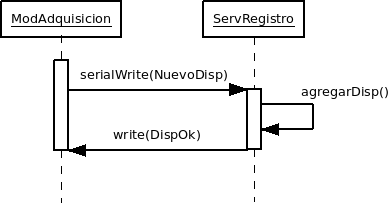
\includegraphics[width=0.5\textwidth,keepaspectratio=true]{img/agregardisp.png}
  \caption{Registro de Nuevo Dispositivo de Adquisición}
  \label{fig:esquema}
 \end{center}
\end{figure}

\newpage
\subsection{\textcolor[gray]{.2}{Diagramas de Actividades}}
% === Figura ====
\begin{figure}[h!]
 \begin{center}
  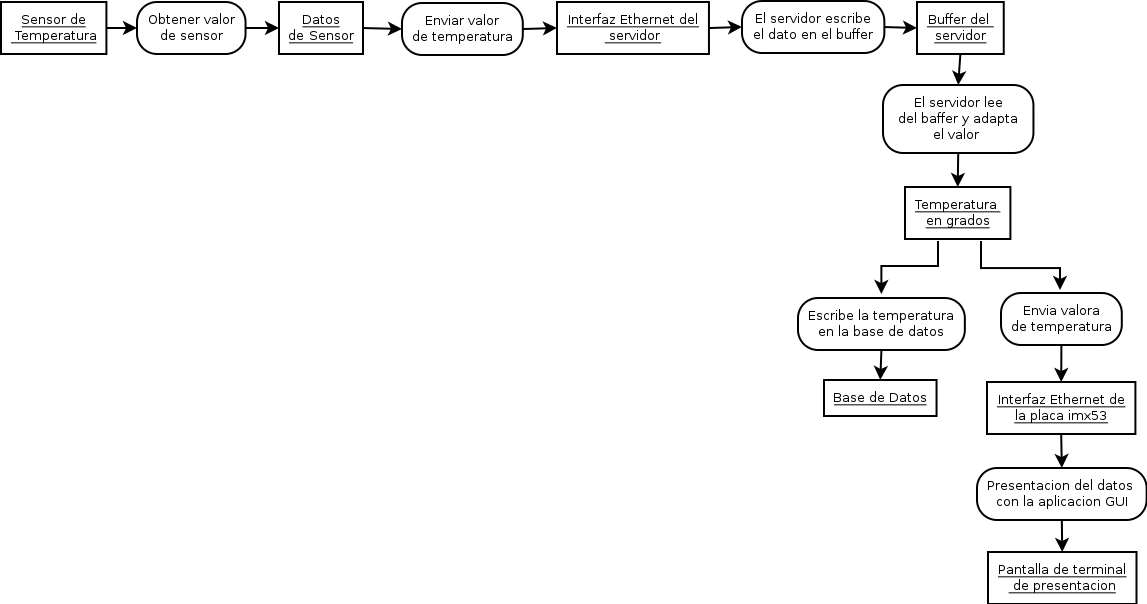
\includegraphics[width=1\textwidth,keepaspectratio=true]{img/diagactiv.png}
 \caption{Flujo de Dato de Temperatura del Sistema}
  \label{fig:esquema}
 \end{center}
\end{figure}


\subsection{\textcolor[gray]{.2}{Diagramas de Casos de Uso}}
\begin{figure}[h!]
 \begin{center}
  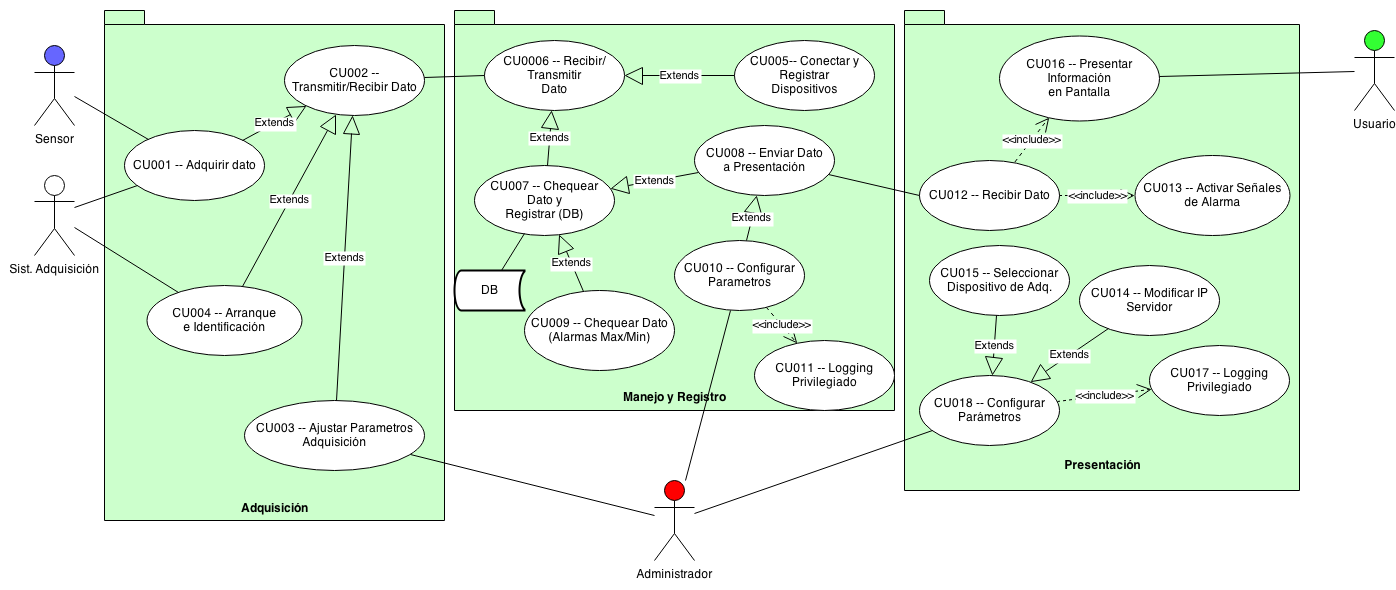
\includegraphics[width=1\textwidth,keepaspectratio=true]{img/usecases.png}
  \caption{Diagrama General de Casos de Uso}
  \label{fig:esquema}
 \end{center}
\end{figure}

\newpage
\subsection{\textcolor[gray]{.2}{LEL – Léxico Extendido del Lenguaje}}
	
		\begin{table}[h!]
		\centering
		\begin{tabular}{>{\columncolor[gray]{.8}} p{4cm} |p{9.5cm} }
		\hline
		Sinónimo  & Sensor DTH  \\
		\hline
		Noción & Entidad que adquiere y envía datos \\
		\hline
		Impacto & Envía datos al sistema de adquisición en respuesta a una solicitud \\
		\hline
		\end{tabular}
		\caption{Entrada de LEL :  Sensor DTH }
		%\label{tab:requsr1}
		\end{table}

\begin{table}[h!]
		\centering
		\begin{tabular}{>{\columncolor[gray]{.8}} p{4cm} |p{9.5cm} }
		\hline 
		Sinónimo  & Sistema de adquisición  \\
		\hline
		Noción & Entidad que solicita, recibe y envía datos \\
		\hline
		Impacto & \begin{itemize}
					 \item Solicita datos al sensor  
					 \item Recibe datos del sensor 
					 \item Establece conexión con el servidor
					 \item Envía datos al sistema de manejo y registro de datos en respuesta a una solicitud
					\end{itemize}\\
		\hline
		\end{tabular}
		\caption{Entrada de LEL : Sistema de adquisición}
		%\label{tab:requsr1}
		\end{table}

\begin{table}[h!]
		\centering
		\begin{tabular}{>{\columncolor[gray]{.8}} p{4cm} |p{9.5cm} }
		\hline
		Sinónimo  & Sistema de manejo y registro de datos  \\
		\hline
		Noción & Entidad que recibe, convierte, almacena y reenvía datos  \\
		\hline
		Impacto & \begin{itemize}
					 \item Solicita datos al sistema de adquisición   
					 \item Recibe datos del sistema de adquisición
					\item  Almacena datos en su base de datos
					 \item Establece conexión con el sistema de adquisición y el sistema de presentación de datos
					 \item Envía datos al sistema de presentación de datos en respuesta a una solicitud
					\end{itemize}\\ 
		\hline
		\end{tabular}
		\caption{Entrada de LEL :  Sistema de manejo y registro de datos }
		%\label{tab:requsr1}
		\end{table}

\newpage
\begin{table}[h!]
		\centering
		\begin{tabular}{>{\columncolor[gray]{.8}} p{4cm} |p{9.5cm} }
		\hline
		Sinónimo  & Sistema de presentación de datos  \\
		\hline
		Noción & Entidad que recibe, convierte, almacena y reenvía datos  \\
		\hline
		Impacto & \begin{itemize}
					 \item Solicita datos al sistema de manejo y registro   
					 \item Recibe datos del sistema de manejo y registro
					 \item Establece conexión con el sistema de manejo y registro de datos
					 \item Envía condiciones de alarmas al sistema de registro y manejo de datos.
					\end{itemize}\\ 
		\hline
		\end{tabular}
		\caption{Entrada de LEL : Sistema de manejo y registro de datos}
		%\label{tab:requsr1}
		\end{table}

		\begin{table}[h!]
		\centering
		\begin{tabular}{>{\columncolor[gray]{.8}} p{4cm} |p{9.5cm} }
		\hline
		Sinónimo  & Usuario  \\
		\hline
		Noción &   Entidad que consulta datos en el sistema de presentación\\
		\hline
		Impacto & 	\begin{itemize}
						\item Visualiza datos en el módulo de presentación
						\item Visualiza señales de alarma ante datos fuera de rango
					\end{itemize}\\
		\hline
		\end{tabular}
		\caption{Entrada de LEL : Usuario}
		%\label{tab:requsr1}
		\end{table}


		\begin{table}[h!]
		\centering
		\begin{tabular}{>{\columncolor[gray]{.8}} p{4cm} |p{9.5cm} }
		\hline
		Sinónimo  & Administrador  \\
		\hline
		Noción &   Entidad que configura los sistemas de adquisición, manejo \& registro y presentación de datos\\
		\hline
		Impacto & 	\begin{itemize}
						\item Ajusta parámetros de adquisición : Intervalo de adquisición , sensores conectados, etc.
						\item Configura parámetros de manejo y registro: Ajusta unidades de medida registrada, intervalo de registro , etc.
						\item Establece parámetros de presentación: Puntos máximos y mínimos de alarmas, unidad de medida presentada, sensores presentados, etc.
					\end{itemize}\\
		\hline
		\end{tabular}
		\caption{Entrada de LEL : Administrador}
		%\label{tab:requsr1}
		\end{table}


\newpage
\subsection{\textcolor[gray]{.2}{Escenarios}}

		\begin{table}[h!]
		\centering
		\begin{tabular}{>{\columncolor[gray]{.8}} p{4cm} |p{9.5cm} }
		\hline
		Título  & Adquirir dato\\
		\hline
		Objetivo &  Adquirir dato del sensor al módulo de adquisición presente en Arduino \\
		\hline
		Contexto & Conexión establecida entre el sensor y el sistema de adquisición\\
		\hline
		Recursos &  Sensor y Arduino (Módulo de adquisición)\\
		\hline
		Actores &  Sensor , Sistema de adquisición\\
		\hline
		Episodios &  \begin{itemize}
						\item El sistema de adquisición establece conexión con el sensor conectado
						\item El sist. de adquisición solicita un dato al sensor conectado
						\item El sensor envía el dato solicitado al sistema de adquisición
						\item El sistema de adquisición recibe el dato del sensor.
					\end{itemize} \\		
		\hline
		\end{tabular}
		\caption{Escenario : Adquirir dato}
		%\label{tab:requsr1}
		\end{table}

\begin{table}[h!]
		\centering
		\begin{tabular}{>{\columncolor[gray]{.8}} p{4cm} |p{9.5cm} }
		\hline
		Título  & Recibir y registrar dato\\
		\hline
		Objetivo &  Recibir dato del módulo de adquisición y registrarlo en la base de datos \\
		\hline
		Contexto & Conexión establecida entre el módulo de adquisición y el sistema de manejo y registro de datos\\
		\hline
		Recursos &  Sistema de adquisición,Sistema de manejo y registro de datos, Base de datos\\
		\hline
		Actores & Sistema de adquisición, Sistema de manejo y registro\\
		\hline
		Episodios &  \begin{itemize}
						\item El sistema de manejo y registro establece conexión con el sistema de adquisición
						\item El sist. de manejo y registro solicita un dato al sistema de adquisición
						\item El sistema de adquisición envía el dato solicitado al sistema de manejo y registro
						\item El sistema de Manejo y registro recibe el dato, lo adapta y almacena en la base de datos.
					\end{itemize} \\	
		\hline
		\end{tabular}
		\caption{Escenario : Recibir y registrar dato}
		%\label{tab:requsr1}
		\end{table}


\begin{table}[h!]
		\centering
		\begin{tabular}{>{\columncolor[gray]{.8}} p{4cm} |p{9.5cm} }
		\hline
		Título  & Presentar datos\\
		\hline
		Objetivo &  Presentar al usuario los datos obtenidos del sistema de manejo y registro\\
		\hline
		Contexto & Conexión establecida entre el módulo de manejo \& registro y el sistema de presentación\\
		\hline
		Recursos &  Sistema de manejo y registro de datos, sistema de presentación\\
		\hline
		Actores & Sistema de manejo y registro, sistema de presentación, usuario\\
		\hline
		Episodios &  \begin{itemize}
						\item El sistema de presentación establece conexión con el sistema de manejo y registro
						\item El sistema de presentación solicita un dato al sistema de manejo y registro
						\item El sistema de manejo y registro envía el dato solicitado al sistema de presentación
						\item El sistema de presentación recibe el dato, lo adapta y lo presenta al usuario gráficamente.
					\end{itemize} \\	
		\hline
		\end{tabular}
		\caption{Escenario: Presentar dato}
	%\label{tab:requsr1}
		\end{table}

\clearpage
\subsection{\textcolor[gray]{.2}{Tarjetas CRC}}
 
 Con lo planteado anteriormente en LEL y los escenarios planteados se generan las siguientes clases candidatas:
 		
 		\begin{table}[h!]
 		\centering
 		\begin{tabular}{>{\columncolor[gray]{.8}} p{4cm} |p{9.5cm} }
		\hline
		Tarjeta CRC primaria & ServidorManejoyRegistro \\
 		\hline
 		Responsabilidades & \begin{itemize}
 								\item Solicita el envío de datos al sistema de adquisición 
 								\item Recibe datos del sistema de adquisición
 								\item Almacena datos en su base de datos
 								\item Establece conexión con el sistema de adquisición el sistema de presentación de datos
 								\item Envía datos al sistema de presentación de datos en respuesta a una solicitud
 							 \end{itemize} \\	
 		\hline
 		Colaboradores &  Sistema de adquisición , sistema de presentación de datos\\
 		\hline
 		\end{tabular}
 		\caption{CRC primaria ServidorManejoyRegistro}
 	%\label{tab:requsr1}
 		\end{table}

		\begin{table}[h!]
		\centering
		\begin{tabular}{>{\columncolor[gray]{.8}} p{4cm} |p{9.5cm} }
		\hline
		Tarjeta CRC primaria & ClientePresentación\\
		\hline
		Responsabilidades & \begin{itemize}
							\item Solicita datos al sistema de manejo y registro
							\item Recibe datos del sistema de manejo y registro
							\item Establece conexión con el sistema de manejo y registro de datos
							\item Envía condiciones de alarmas al sistema de registro y manejo de datos
							\end{itemize} \\
		\hline
		Colaboradores & sistema de manejo y registro de datos, administrador y usuario\\

		\hline
		\end{tabular}
		\caption{CRC primaria ClientePresentación}
	%\label{tab:requsr1}
		\end{table}

		\begin{table}[h!]
		\centering
		\begin{tabular}{>{\columncolor[gray]{.8}} p{4cm} |p{9.5cm} }
		\hline
		Tarjeta CRC secundarias & ClienteConexión\\
		\hline
		Responsabilidades & \begin{itemize}
								\item Establecer la conexión con el sistema de registro y manejo de datos
								\item Envío de datos datos al sistema de registro y manejo de datos
							 \end{itemize} \\
		\hline
		Colaboradores &  Sensor, sistema de adquisición \\
		\hline
		\end{tabular}
		\caption{CRC secundaria ClienteConexión}
	%\label{tab:requsr1}
		\end{table}

		\begin{table}[h!]
		\centering
		\begin{tabular}{>{\columncolor[gray]{.8}} p{4cm} |p{9.5cm} }
		\hline
		Tarjeta CRC secundaria & ConexiónServidor\\
		\hline
		Responsabilidades & \begin{itemize}
								\item Establecer la conexión con el sistema de adquisición
								\item Establecer la conexión con el sistema de presentación
								\item Recibir datos del sistema de adquisición
								\item Enviar datos al módulo de presentación
							 \end{itemize} \\
		\hline
		Colaboradores& Sistema de manejo y registro , Sistema de adquisición\\
		\hline
		\end{tabular}
		\caption{Tarjeta CRC secundaria ConexiónServidor}
	%\label{tab:requsr1}
		\end{table}

		\begin{table}[h!]
		\centering
		\begin{tabular}{>{\columncolor[gray]{.8}} p{4cm} |p{9.5cm} }
		\hline
		Tarjeta CRC secundaria & BaseDeDatos\\
		\hline
		Responsabilidades & \begin{itemize}
								\item Establecer conexión con el gestor de base de datos
								\item Registrar datos recibidos del sistema de adquisición
								 \end{itemize} \\
		\hline
		Colaboradores& Sistema de adquisición \\

		\hline
		\end{tabular}
		\caption{Tarjeta CRC secundaria BaseDeDatos}
	%\label{tab:requsr1}
		\end{table}


		\begin{table}[h!]
		\centering
		\begin{tabular}{>{\columncolor[gray]{.8}} p{4cm} |p{9.5cm} }
		\hline
		Tarjeta CRC secundaria & ConexiónClienteVista\\
		\hline
		Responsabilidades & \begin{itemize}
								\item Establecer conexión con el sistema de manejo y registro
								\item Recibir datos del sistema de manejo y recepción
								\item Enviar mensajes de estado de alarmas al sistema de manejo y registro de datos
							 \end{itemize} \\
		\hline
		Colaboradores& Sistema de presentación , Sistema de manejo y registro\\
		\hline

		\end{tabular}
		\caption{Escenario: Presentar dato}
	%\label{tab:requsr1}
		\end{table}

		\begin{table}[h!]
		\centering
		\begin{tabular}{>{\columncolor[gray]{.8}} p{4cm} |p{9.5cm} }
		\hline
		Tarjeta CRC secundaria & VistaDatos\\
		\hline
		Responsabilidades & \begin{itemize}
								\item Mostrar gráficamente los datos recibidos del módulo de manejo y registro
								\item Mostrar estado de alarmas de valor mínimo y máximo
								 \end{itemize} \\
		\hline
		Colaboradores& Sistema de presentación \\
		\hline
		\end{tabular}
		\caption{Tarjeta CRC secundaria VistaDatos}
	%\label{tab:requsr1}
		\end{table}



\chapter{\textcolor[gray]{.8}{ADD - ARCHITECTURAL DESIGN DOCUMENT}}
\newpage
<<<<<<< HEAD
%\section{\textcolor{orange}{Historial de Versiones}}
%\begin{table}[!h]
%\begin{center}
%\begin{tabular}{|c|c|c|c|}
%\hline
%\rowcolor[RGB]{255,127,0} Vesión & Fecha & Descripción de Cambios & Autor\\
%\hline
%1.0 & 15/09/2013 & Primera Versión & Lovaisa V.\\
%\hline
%\end{tabular}
%\end{center}
%\end{table}
%\newpage

%\section{\textcolor{orange}{Página de Aprobaciones}}
%A continuación se listan las personas de las cuales se requiere la aceptación de
%cualquier cambio mayor de este documento.
%\begin{enumerate}
 % \item Estas aprobaciones no son necesarias si el cambio es menor.
  %\item Estas aprobaciones son necesarias si el cambio es realizado por alguna
  %persona distinta de ellas.
%\end{enumerate}
%\begin{table}[!h]
%\begin{center}
%\begin{tabular}{|c|c|c|c|}
%\hline
%\rowcolor[RGB]{255,127,0} Nombre & Cargo & Fecha & Firma\\
%\hline
%Lovaisa Valeria & Resp. Diseño Arquitectónico & 15/09/2013 & \\
%\hline
%Gomez Pablo & Resp. Suplente & 15/09/2013 & \\
%\hline
%\end{tabular}
%\end{center}
%\end{table}

%\newpage
\section{\textcolor{orange}{Introducción}}
\subsection{\textcolor{orange}{Propósito y Alcance}}
=======
\section{\textcolor[gray]{.2}{Historial de Versiones}}
\begin{table}[!h]
\begin{center}
\begin{tabular}{|c|c|c|c|}
\hline
\rowcolor[gray]{.8} Vesión & Fecha & Descripción de Cambios & Autor\\
\hline
1.0 & 15/09/2013 & Primera Versión & Lovaisa V.\\
\hline
\end{tabular}
\end{center}
\end{table}
\newpage

\section{\textcolor[gray]{.2}{Página de Aprobaciones}}
A continuación se listan las personas de las cuales se requiere la aceptación de
cualquier cambio mayor de este documento.
\begin{enumerate}
  \item Estas aprobaciones no son necesarias si el cambio es menor.
  \item Estas aprobaciones son necesarias si el cambio es realizado por alguna
  persona distinta de ellas.
\end{enumerate}
\begin{table}[!h]
\begin{center}
\begin{tabular}{|c|c|c|c|}
\hline
\rowcolor[gray]{.8} Nombre & Cargo & Fecha & Firma\\
\hline
Lovaisa Valeria & Resp. Diseño Arquitectónico & 15/09/2013 & \\
\hline
Gomez Pablo & Resp. Suplente & 15/09/2013 & \\
\hline
\end{tabular}
\end{center}
\end{table}

\newpage
\section{\textcolor[gray]{.2}{Introducción}}
\subsection{\textcolor[gray]{.2}{Propósito y Alcance}}
>>>>>>> 3910ab7b9e4c32b7e12f785ce015e1bd7260973a
Este documento cubre el diseño de la arquitectura  del sistema
de monitoreo y registro de datos multipropósito. Este ADD tiene como objetivo
esteblecer la arquitectura del sistema , sus componentes , patrones
arquitéctonicos utilizados para luego ser implementados en la etapa de desarrollo.

\subsection{\textcolor[gray]{.2}{Acrónimos y Glosario}}
\begin{table}[!h]
\begin{center}
\begin{tabular}{|c|c|}
\hline
\rowcolor[gray]{.8} Acrónimo & Descripción \\
\hline
ADD & Architectural Design Document – Documento de diseño de arquitectura\\
\hline
ADM & Architectural Design Manager – Responsable de diseño de arquitectura\\
\hline
MVC & Model view controller – Modelo vista controlador (Patrón de
Arquitectura)\\
\hline
\end{tabular}
\end{center}
\end{table}

\subsection{\textcolor[gray]{.2}{Herramientas Necesarios}}
\begin{table}[!h]
\begin{center}
\begin{tabular}{|c|p{100mm}|}
\hline
\rowcolor[gray]{.8} Programa & Propósito \\
\hline
Dia & Software para la creación de diagramas UML \\
\hline
\end{tabular}
\end{center}
\end{table}

<<<<<<< HEAD
%\newpage
%\section{\textcolor{orange}{Roles}}
%\subsection{\textcolor{orange}{Responsables}}
%Las actividades de ingeniería de requerimientos del Sistema serán coordinadas en
%este proyecto por el Responsable de Requerimientos del sistema. (SRM). Este Rol
%debe ser asignado a alguno de los miembros del proyecto.
%El SRM será el responsable directo de las actividades de requerimientos delsistema, responder ante modificaciones en los mismos  y de mantener la documentación relacionada actualizada (Modificación de requerimientos , Matriz de Trazabilidad , Modificación del sistema de trackeo).


%\subsection{\textcolor{orange}{Roles}}
%\begin{table}[!h]
%\begin{center}
%\begin{tabular}{|c|c|c|}
%\hline
%\rowcolor[RGB]{255,127,0} Rol & Nombre & Suplente\\
%\hline
%ADM & Lovaisa Valeria & Gomez Pablo\\
%\hline
%\end{tabular}
%\end{center}
%\end{table}
=======
\newpage
\section{\textcolor[gray]{.2}{Roles}}
\subsection{\textcolor[gray]{.2}{Responsables}}
Las actividades de ingeniería de requerimientos del Sistema serán coordinadas en
este proyecto por el Responsable de Requerimientos del sistema. (SRM). Este Rol
debe ser asignado a alguno de los miembros del proyecto.
El SRM será el responsable directo de las actividades de requerimientos del
sistema, responder ante modificaciones en los mismos  y de mantener la
documentación relacionada actualizada (Modificación de requerimientos , Matriz
de Trazabilidad , Modificación del sistema de trackeo).


\subsection{\textcolor[gray]{.2}{Roles}}
\begin{table}[!h]
\begin{center}
\begin{tabular}{|c|c|c|}
\hline
\rowcolor[gray]{.8} Rol & Nombre & Suplente\\
\hline
ADM & Lovaisa Valeria & Gomez Pablo\\
\hline
\end{tabular}
\end{center}
\end{table}
>>>>>>> 3910ab7b9e4c32b7e12f785ce015e1bd7260973a

\newpage
\section{\textcolor[gray]{.2}{Diseño Preliminar}}
\subsection{\textcolor[gray]{.2}{Diagrama Preliminar de Diseño de Arquitectura}}
\begin{figure}[h!]
 \begin{center}
  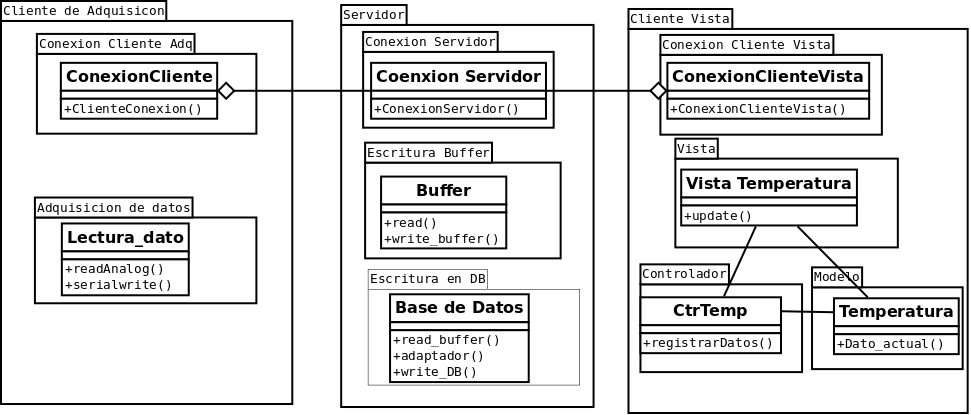
\includegraphics[width=1\textwidth,keepaspectratio=true]{./img/arqprelim.png}
  \caption{Arquitectura Preliminar}
  \label{fig:esquema}
 \end{center}
\end{figure}

\subsection{\textcolor[gray]{.2}{Descripción de la Arquitectura Preliminar}}
Se seleccionó el patrón Cliente–Servidor para atacar el modelo de conexión de
los dispositivos de adquision al servidor del sistema. El servidor será el
encargado de correr las instancias necesarias para atender a cada dispositivo
de aquisición conectado via sockets mediante el protocolo UDP.

El servidor es un Iterator, el cual recibe información de cada uno de los
clientes de adquisión e informa a cada uno de los clientes de presentación los
cambios en el modelo (temperaturas , modificación de alarmas , etc).
Con respecto al cliente Presentación , se tiene una arquitectura MVC
(modelo-vista-controlador) donde se encapsulan los datos  de
temperatura (generados por patrón Observer) en el “Modelo” , mientras que el
modelo gráfico se representa en la “Vista” que posee componentes generados
también con el patrón Observer. Finalmente “Vista” presenta , son atendidas por
los objetos contenidos en el paquete “Controlador” cuyas clases componentes son
generadas con el patrón Observer.

Con la aplicación de esta arquitectura se resuelven los requisitos no funciones
relacionados a las diferentes formas de interactuar con los datos.
Permite vez lograr aplicar sin mayores cambios futuros requerimientos para la
interacción y presentación de los datos.

Respecto al modelo Cliente – Servidor aplicado en la conexión este se
aplica ya que varios dispositivos deben conectarse al sistema  desde diferentes
ubicaciones. Y deben acceder a datos compartidos . En este caso los sitemas se
distribuye en una red LAN y debe estar disponible para todos los dispositivos de
presentacion que se encuentren en dicha red.

El funcionalidad del servidor es aceptar peticiones de conexión de dispositivos
de adqucion y presentación de datos, registrar datos en la base de tados
adaptados para una lectura apropiada.

\newpage
\section{\textcolor[gray]{.2}{Contexto del sistema}}
\subsection{\textcolor[gray]{.2}{Diagrama de Despliegue}}
\begin{figure}[h!]
 \begin{center}
  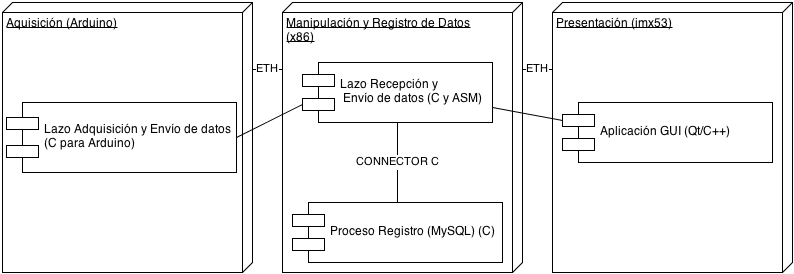
\includegraphics[width=1\textwidth,keepaspectratio=true]{img/Deployement.png}
  \caption{Diagrama de Despliegue del Sistema}
  \label{fig:esquema}
 \end{center}
\end{figure}

\subsection{\textcolor[gray]{.2}{Descripción del contexto del sistema}}

EL subsistema de Adquisición  de datos que se encuentra corriendo sobre una plataforma hardware arduino, envía datos de temperatura por medio de la interfaz Ethernet obtenidos mediante el instrumento adecuado para esto(sensor de temperatura),después de haberse identificado correctamente con el subsistema de manipulación y registro de datos el cual tendrá el rol de servidor sobre una plataforma hardware X86,donde se registran los datos de temperatura en una base de datos, mientras que el subsistema de presentación de datos que se encuentra corriendo en una plataforma hardware imx53 debidamente identificado con el servidor, es el encargado por medio de una conexión Ethernet, mostrar el dato de temperatura a través de un interfaz gráfica al usuario. 
Esta decisión de arquitectura se basa en el requerimiento funcional que especifica que el subsitema de de adquisición, registro, manipulación y presentación de datos  deben cumplir con una arquitectura Cliente-Servidor. 

\newpage


\chapter{\textcolor[gray]{.2}{SDD - SOFTWARE DESINGN DESCRIPTION}}
%\newpage
%\section{\textcolor[gray]{.2}{Historial de Versiones}}
%\begin{table}[!h]
%\begin{center}
%\begin{tabular}{|c|c|c|c|}
%\hline
%\rowcolor[gray]{.8} Vesión & Fecha & Descripción de Cambios & Autor\\
%\hline
%1.0.0 & 09/07/2013 & Primera Versión del diseño del Sist. & Gomez P.\\
%\hline
%1.0.1 & 12/07/2013 & Descripciòn bàsica de patrones implementados & Lovaisa V.\\
%\hline
%\end{tabular}
%\end{center}
%\end{table}
%\newpage
%
%\section{\textcolor[gray]{.2}{Página de Aprobaciones}}
%A continuación se listan las personas de las cuales se requiere la aceptación de
%cualquier cambio mayor de este documento.
%\begin{enumerate}
%  \item Estas aprobaciones no son necesarias si el cambio es menor.
%  \item Estas aprobaciones son necesarias si el cambio es realizado por alguna
%  persona distinta de ellas.
%\end{enumerate}
%\begin{table}[!h]
%\begin{center}
%\begin{tabular}{|c|c|c|c|}
%\hline
%\rowcolor[gray]{.8} Nombre & Cargo & Fecha & Firma\\
%\hline
%Lovaisa Valeria & Resp. Diseño & 09/07/2013 & \\
%\hline
%Gomez Pablo & Resp. Suplente & 15/07/2013 & \\
%\hline
%\end{tabular}
%\end{center}
%\end{table}

\newpage
\section{\textcolor[gray]{.2}{Introducción}}
\subsection{\textcolor[gray]{.2}{Propósito y Alcance}}
Este documento cubre el diseño del sistemade monitoreo y registro de datos multipropósito. Este SDD tiene como objetivo establecer el diseño del sistema , sus componentes , patrones utilizados y lo todo lo relacionado a la etapa de diseño que añada detalles para su implementación. 

\subsection{\textcolor[gray]{.2}{Acrónimos y Glosario}}
\begin{table}[!h]
\begin{center}
\begin{tabular}{|c|c|}
\hline
\rowcolor[gray]{.8} Acrónimo & Descripción \\
\hline
SDD & Software Design Document - Documento de diseño del sistema. \\
\hline
SDM & Software Design Manager – Responsable de diseño del sistema\\
\hline
\end{tabular}
\end{center}
\end{table}

\subsection{\textcolor[gray]{.2}{Herramientas Necesarios}}
\begin{table}[!h]
\begin{center}
\begin{tabular}{|c|p{100mm}|}
\hline
\rowcolor[gray]{.8} Programa & Propósito \\
\hline
Google Driver & Software necesario para llevar los documentos de diseño empleados.\\
%de requermientos usr. vs req. de sistema y de req. vs casos de uso.\\
\hline
Dia & Software para la creación de diagramas UML\\
\hline
Git-Hub & Software necesario para llevar el control de versiones del código \\
\hline
\end{tabular}
\end{center}
\end{table}

%\newpage
%\section{\textcolor[gray]{.2}{Roles}}
%\subsection{\textcolor[gray]{.2}{Responsables}}
%
%Las actividades de Diseño del Sistema serán coordinadas en este proyecto por el Responsable de diseño de sistema. (SDM). Este Rol debe ser asignado a alguno de los miembros del proyecto.
%El SDM será el responsable directo de las actividades de diseño, responder ante modificaciones en la misma  y de mantener la documentación relacionada actualizada.
%
%
%\subsection{\textcolor[gray]{.2}{Roles}}
%\begin{table}[!h]
%\begin{center}
%\begin{tabular}{|c|c|c|}
%\hline
%\rowcolor[gray]{.8} Rol & Nombre & Suplente\\
%\hline
%SRM & Gomez Pablo & Lovaisa Valeria\\
%\hline
%\end{tabular}
%\end{center}
%\end{table}

\newpage
\section{\textcolor[gray]{.2}{Vista general del diseño}}
\subsection{\textcolor[gray]{.2}{Diagrama de paquetes}}
% === Figura ====
\begin{figure}[h!]
 \begin{center}
  \includegraphics[width=1\textwidth,keepaspectratio=true]{img/diagrama_paquetes.png}
 %\caption{Flujo de Dato de Temperatura del Sistema}
  \label{fig:esquema}
 \end{center}
\end{figure}
% ===============
%\subsection{\textcolor[gray]{.2}{Diagrama de clases paquetes Cliente-Aquisiciòn de Datos}}


\subsection{\textcolor[gray]{.2}{Diagrama de clases paquetes Cliente-Presentaciòn de Datos}}


%\subsection{\textcolor[gray]{.2}{Diagrama de clases paquetes Servidor}}
% === Figura ====
\begin{figure}[h!]
 \begin{center}
  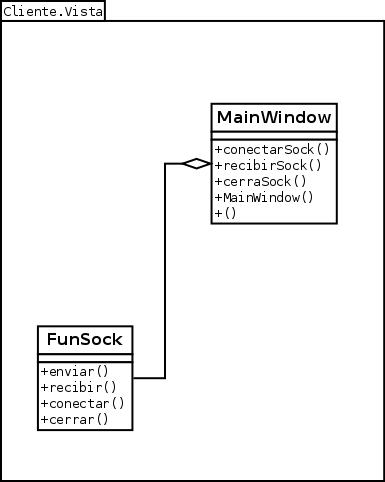
\includegraphics[width=0.5\textwidth,keepaspectratio=true]{img/Clases_Vista.png}
 %\caption{Flujo de Dato de Temperatura del Sistema}
  \label{fig:esquema}
 \end{center}
\end{figure}
% ===============



\section{\textcolor[gray]{.2}{Patrones Implementados}}
\subsection{\textcolor[gray]{.2}{Patròn Observer }}

Este patrón se utiliza cuando un conjunto de sensores se monitoriza y despliega de manera rutinaria. En el momento en que los sensores indican que sucedió cierto evento, el sistema reacciona iniciando un proceso para manejar dicho evento.
El sensor de temperatura DTH11 rutinariamente toma cada 1seg un nuevo dato de temperatura  y lo envía a través de una interfaz Ethernet a un servidor

\subsection{\textcolor[gray]{.2}{Patrón Ambiental}}

Este patrón se emplea cuando un sistema incluye sensores que proporcionan información sobre el entorno y los actuadores que pueden cambiar el entorno. En respuesta a los cambios ambientales detectados por el sensor, se envían señales de control a los actuadores del sistema.

El sensor de temperatura toma la temperatura del el entorno y el servidor verifica que los valores medidos se encuentren dentro de el rango establecido, en el caso de no cumplir con los valores mínimos y máximos de temperatura pre establecidos el servidor lanza una alarma que se puede visualizar en el monitor conectado en de la terminal de la plataforma hardware iMx53.

 
\subsection{\textcolor[gray]{.2}{Segmentaciòn de Proceso(process pipeline)}}

Este patrón se usa al transformarse datos de una representación a otra antes de que puedan procesarse. La transformación se implementa como una secuencia de pasos de procesamiento, que puede realizarse de manera concurrente. Esto permite un procesamiento de datos muy rápido, debido a un núcleo o procesador separado puede ejecutar cada transformación.

El proceso productor en el servidor recibe por medio de la interfaz Ethernet el dato de temperatura y lo graba en un buffer circular en memoria compartida donde el proceso consumidor toma el dato lo procesa, lo registra en una base de datos y lo envía a través de la interfaz Ethernet para ser presentado


\chapter{\textcolor[gray]{.8}{STD - SOFTWARE TEST DOCUMENTATION}}
\newpage
\section{\textcolor[gray]{.2}{Historial de Versiones}}
\begin{table}[!h]
\begin{center}
\begin{tabular}{|c|c|c|c|}
\hline
\rowcolor[gray]{.8} Vesión & Fecha & Descripción de Cambios & Autor\\
\hline
1.0.0 & 12/09/2013 & Primera Versión del documento de testing del sistema & Lovaisa V.\\
\hline
1.0.1 & 14/09/2013 & Se establece Criterio de Aceptación , Req mínimos cant de UTs y STs & Gomez P.\\
\hline
1.0.2 & 15/09/2013 & Se actualizan las Pruebas de Sistema & Gomez P.\\
\hline
\end{tabular}
\end{center}
\end{table}
\newpage

\section{\textcolor[gray]{.2}{Página de Aprobaciones}}
A continuación se listan las personas de las cuales se requiere la aceptación de cualquier cambio mayor de este documento.
\begin{enumerate}
  \item Estas aprobaciones no son necesarias si el cambio es menor.
  \item Estas aprobaciones son necesarias si el cambio es realizado por alguna
  persona distinta de ellas.
\end{enumerate}
\begin{table}[!h]
\begin{center}
\begin{tabular}{|c|c|c|c|}
\hline
\rowcolor[gray]{.8} Nombre & Cargo & Fecha & Firma\\
\hline
Lovaisa Valeria & Resp. Testing & 12/09/2013 & \\
\hline
Gomez Pablo & Resp. Suplente & 12/09/2013 & \\
\hline
\end{tabular}
\end{center}
\end{table}

\newpage
\section{\textcolor[gray]{.2}{Introducción}}
\subsection{\textcolor[gray]{.2}{Propósito y Alcance}}
Este documento cubre el proceso de prueba del sistema de monitoreo y registro de datos multipropósito. Este STD tiene como objetivo establecer cuales seràn los casos de pruebas que se realizaràn y como deberàn documentarse los resultados obtenidos.

\subsection{\textcolor[gray]{.2}{Acrónimos y Glosario}}
\begin{table}[!h]
\begin{center}
\begin{tabular}{|c|c|}
\hline
\rowcolor[gray]{.8} Acrónimo & Descripción \\
\hline
STD & Software Test Document - Documento de prueba del sistema. \\
\hline
STM & Software Testing Manager – Responsable de prueba del sistema\\
\hline
\end{tabular}
\end{center}
\end{table}

\subsection{\textcolor[gray]{.2}{Herramientas Necesarios}}
\begin{table}[!h]
\begin{center}
\begin{tabular}{|c|p{100mm}|}
\hline
\rowcolor[gray]{.8} Programa & Propósito \\
\hline
Google Driver & Software necesario para llevar los documentos de diseño empleados.\\
%de requermientos usr. vs req. de sistema y de req. vs casos de uso.\\
\hline
Dia & Software para la creación de diagramas UML\\
\hline
Git-Hub & Software necesario para llevar el control de versiones del código y los documentos de prueba empleados.\\
\hline
CUnit plugin & SPlug-in necesario para el desarrollo de pruebas unitarias.\\
\hline
\end{tabular}
\end{center}
\end{table}

\newpage
\section{\textcolor[gray]{.2}{Roles}}
\subsection{\textcolor[gray]{.2}{Responsables}}

Las actividades de pruebas del Sistema serán coordinadas en este proyecto por el Responsable de pruebas del sistema. (STM). Este Rol debe ser asignado a alguno de los miembros del proyecto.

El STM será el responsable directo de las actividades de testing, responder ante modificaciones en las mismas  y de mantener la documentación relacionada actualizada.



\subsection{\textcolor[gray]{.2}{Roles}}
\begin{table}[!h]
\begin{center}
\begin{tabular}{|c|c|c|}
\hline
\rowcolor[gray]{.8} Rol & Nombre & Suplente\\
\hline
STM & Lovaisa Valeria & Gomez Pablo\\
\hline
\end{tabular}
\end{center}
\end{table}

\newpage
\section{\textcolor[gray]{.2}{Plan de pruebas - Test Plan}}
\subsection{\textcolor[gray]{.2}{Descripción de la herramientas utilizada}}

Se utilizará la herramienta CUnit integrada a Netbeans. Esta herramienta permitirá obtener el Pass/Fail ratio , determinar paquetes de UT a correr como Sanity Tests e  identificar bugs.

\subsection{\textcolor[gray]{.2}{Elementos a probar - Test elements}}

Se realizarán pruebas unitarias a todos los elementos involucrados en el sistema considerados de importancia significativa por el STM. Deben generarse al menos 3 UT por clase generada incrementando este valor según la importancia de la clase en cuestión (a determinar por el STM).

	Se seleccionarán una serie de UTs , de las clases consideradas por el STM como vitales para el funcionamiento del sistema. Con estos UTs se generán al menos 3 Sanity Tests , los cuales garantizan el funcionamiento adecuado del sistema en su mayor parte.


\subsection{\textcolor[gray]{.2}{Caracterìsticas a probar - Features to be Tested}}

Se deberán realizar pruebas unitarias para todos las nuevas características implementadas (Salvo decisión del STM) . Deben generarse los UTs para cada caso antes de desarrollar la implementación de la nueva funcionalidad. Este enfoque permitirá garantizar una integración de código con la menor tasa de defectos para conservar en todos momento una versión construíble en el repositorio Gib-Hub.

\subsection{\textcolor[gray]{.2}{Características a no probar - Features not to be Tested }}

Solo estarán excluídas de ser probadas las funcionalidades que el STM designe como de baja prioridad. 

\subsection{\textcolor[gray]{.2}{Criterio de aceptación - Item Pass-Fail criteria }}

El sistema debe pasar , el 80 %  de los UTs para ser considerado aceptable. Cualquier porcentaje menor no se encuentra en condiciones de entrega.

El sistema debe cumplir con el 100 % de los STs para ser considerado aceptable. Cualquier porcentaje menor no se adecua a las condiciones de entrega.

\subsection{\textcolor[gray]{.2}{Test de sistema }}

Al sistema se le realizarán las siguientes pruebas de sistema antes de la realización de una entega y cuyos resultados serán informados en su correpondiente Release Note

 %\subsubsection{\textcolor[gray]{.2}{Test de conexion Servidor }}

 \subsubsection{\textcolor[gray]{.2}{Test de conexion Cliente.Adqisición }}

\begin{enumerate}
\item Requerimiento: sistema de manejo y registro de datos debe poder conectarse con uno o varios módulos de adquisición de datos por medio de una conexión serial u Ethernet.
\item Propósito: Comprobar que el servidor recibe datos correctamente desde Arduino.
 
\underline{\textcolor[gray]{.8}{Dependencias}}

\item Configuración: Se conecta el Arduino y se espera que le empiece a pedir datos el servidor.
\item Inicialización: Se inicial una aplicación llamada servidor.
\item Finalización: Dispositivo correctamente conectados se pueden leer los datos de temperatura en la base de datos.   
\item Acciones: Se debe conectar el dispositivo de adquisición a la interfaz Ethernet del servidor, a continuación se lanza la aplicación servidor y se accede a la BD.

\underline{\textcolor[gray]{.8}{Resultados}} 

\item Caso positivo: visualización de los datos de temperatura en la base de datos.
\item Caso negativo: Cualquier error en la generación del proceso de conexión, no ver los resultados obtenidos en la base de datos.

\end{enumerate}

 \subsubsection{\textcolor[gray]{.2}{Test de conexion Cliente.Vista }}
\begin{enumerate}
\item Requerimiento: El modulo de presentación de datos debe poder conectarse con un servidor vía conexión Ethernet.
\item Propósito: Comprobar que el servidor envía el dato de temperatura correctamente a la placa iMx53 y es mostrado en pantalla.

\underline{\textcolor[gray]{.8}{Dependencias}}

\item Configuración: Se conecta la placa iMx53 y se espera tener algún dato para extraer de el  buffer ubicado en el servidor.
\item Inicialización: Se inicial una aplicación llamada servidor.
\item Finalización: Dispositivo correctamente conectados se pueden leer los datos de temperatura en el monitor conectado a la placa iMx53.   
\item Acciones :Se debe conectar el dispositivo de presentación a la interfaz Ethernet del servidor, a continuación se lanza la aplicación servidor y se observa el monitor conectado al la placa iMx53.

\underline{\textcolor[gray]{.8}{Resultados}} 

\item Caso positivo: visualización de los datos de temperatura en el monitor.
\item Caso negativo: Cualquier error en la generación del proceso de conexión, no ve el resultado recibido en la pantalla.

\end{enumerate}


 %\subsubsection{\textcolor[gray]{.2}{Test de envio de datos }}

%\\section{\\textcolor[gray]{.2}{Patrones Implementados}}






\end{document}